\section{Design Principles}
\label{sec:design}

We now present the fundamental design principles of a dataplane
architecture designed to run untrusted, even-driven applications, and
designed to address the specific scalabilty challenges of today's
web-scale applications.


\begin{figure}
\hspace*{-0.25in}\centering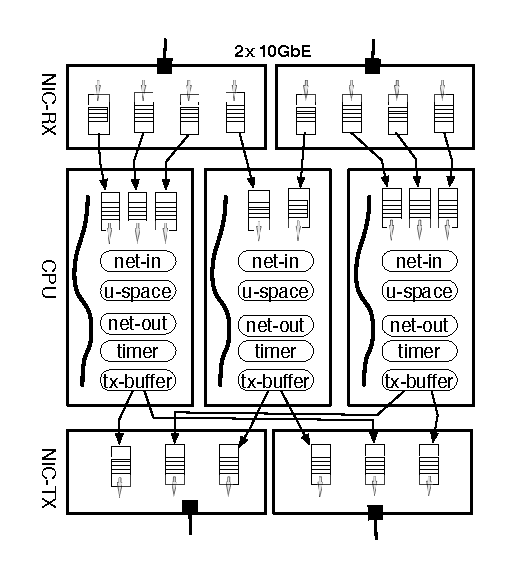
\includegraphics{figs/queues-cores.eps}
\caption{Example of IX scaling across two NICs interfaces, 8 NIC RX queues, and 3 CPU hardware threads.} 
\label{fig:queues-cores}
\end{figure}



\todo Separation of control and data planes.  We use Linux with
real-time priority processes; ensure that interrupts are not directed
to the DP cores (or at least not that much).  Communication mechanism
between control plane and data plane using shared memory (for data)
and sockets (to signal and sleep/wakeup).

\todo Data plane principles

\todo Coherency-free operations  (ala multikernel~\cite{DBLP:conf/sosp/BaumannBDHIPRSS09})

%\todo Dynamic spinning cores : re-define pthread abstraction but use it in a different way

\todo Asynchronous channels (like Megapipe)

\todo Abstraction layers: libevent, libpcap

\todo MORE


